\section{Results}
\subsection{Calibration}
Defects in the geometry of the antenna can lead to the maximum of the sensitivity to not be properly aligned with the pointing of the antenna.


The sun is the strongest discrete radio source in the sky\cite{burke_introduction_2013}. \hl{Le livre a beaucoup de detail sur d'où vient le signal etc}

[aussi \cite{lauterbach_radio_2022} parle du soleil, section 4.1]

\begin{figure}[htbp]
    \centering
    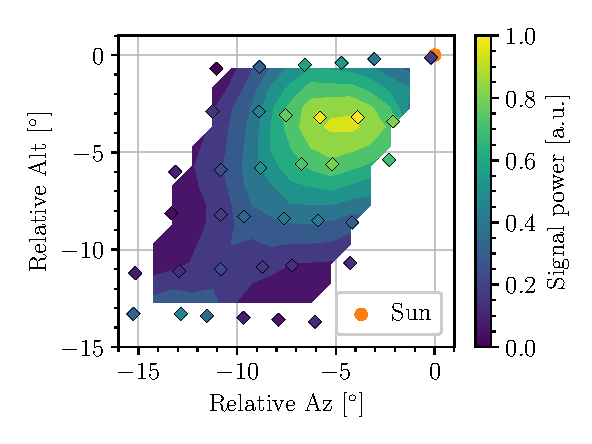
\includegraphics[scale=1]{figures/calibration_contour.pdf}
    \caption{Calibration contour}
    \label{fig:calibration_contour}
\end{figure}

\subsection{Distinguishing signal and noise}
Measure BM building, measure actual H21 source, divide actual by noise to extract the signal from noise, apply some filter and voilà, a nice signal

\subsection{Velocity field of the Milky Way}
Probing arms of milky way

Talk about orientation (i.e. sky visible at measuring time), correct angular momentum?
